
%(BEGIN_QUESTION)
% Copyright 2010, Tony R. Kuphaldt, released under the Creative Commons Attribution License (v 1.0)
% This means you may do almost anything with this work of mine, so long as you give me proper credit

Sketch connecting wires to allow this data acquisition unit (DAQ) to sense strain using quarter-bridge strain gauge circuits on input channels \#1 and \#3, such that increasing tension on the strain gauge (increasing gauge resistance) generates a more {\it positive} signal voltage on each channel:

$$\includegraphics[width=15.5cm]{i04584x01.eps}$$

\vskip 20pt \vbox{\hrule \hbox{\strut \vrule{} {\bf Suggestions for Socratic discussion} \vrule} \hrule}

\begin{itemize}
\item{} Explain why in order for differential DAQ inputs to work, the power supply must share a common connection with the DAQ power supply.
\item{} Explain what the ``AI Gnd'' and ``Shield'' input terminals are generally used for.
\item{} After you have sketched your circuit, evaluate the effects of various components failing either open or shorted, one at a time.
\item{} Identify whether or not {\it bias resistors} are necessary to connect to the DAQ's input terminals.  If so, where should those resistors connect, and what should their approximate sizes be?
\end{itemize}

\underbar{file i04584}
%(END_QUESTION)





%(BEGIN_ANSWER)

\noindent
{\bf Partial answer:}

$$\includegraphics[width=15.5cm]{i04584x03.eps}$$

%(END_ANSWER)





%(BEGIN_NOTES)

Strain gauges increase resistance with increasing tension.  If we want this to make an increasing positive signal for the DAQ to see, we must connect the (+) input to the positive side of the strain gauge, and connect the ($-$) input to the other side of the bridge.

$$\includegraphics[width=15.5cm]{i04584x02.eps}$$

No bias resistors are necessary for the differential DAQ inputs in this application, because the bridge networks provide ample pathways for amplifier bias currents to travel.

%INDEX% Pictorial circuit review (analog signal wiring to data acquisition unit)

%(END_NOTES)

